\documentclass{paper}
\usepackage{float}
\usepackage{graphicx}
\usepackage{hyperref}
\usepackage{amsthm}
\usepackage{amsmath}
\usepackage{amsfonts}
\usepackage[style=authoryear,
    bibstyle=authoryear,
    backend=biber,
    natbib=true,
    maxnames=99,
    maxcitenames=2,
    uniquelist=minyear,
    giveninits=true,
    uniquename=mininit
]{biblatex}

\addbibresource{bibliography.bib}
\graphicspath{{./images}}

\title{Användning av FPGA inom post-kvant kryptografi}
\author{Viktor Horsmanheimo}
\date{\today}

\newtheorem{definition}{Definition}
\newcommand{\bR}{\mathbb{R}}
\newcommand{\bZ}{\mathbb{Z}}

\begin{document}
\maketitle

Kryptografiska system är ofta implementerade inom mjukvara, men under de
senaste decennierna har \textit{Field Programmable Gate Arrays} (FPGA) blivit
allt mer populära inom kryptografi. FPGAn är omprogrammerbar hårdvara som
använder sig av Booleska funktioners egenskaper. Där kan man representera
vilken som helst funktion med hjälp av en sanningstabell. FPGAn implementerar
dessa tabeller i så kallade \textit{uppslagstabeller} (UT). Då funktionen behöver
omprogrameras ändrar man på värden i tabellerna.

Orsaken till att FPGAn har blivit populära är bland annat att i
mjukvaroimplementation av kryptografiska system existerar det flera
attackvektorer, till exempel operativsystemet. Processorn är även en
attackvektor. Detta insåg man med Spectre, som utnyttjade processorns
spekulativa grenförutsägelse. Vi kan använda oss av FPGAn för att separera
krypteringssystemet, vilket minimerar attackvektorerna. Man kan skapa ett
system där mjukvaran aldrig kan komma åt de kryptografiska nycklarna.
% TODO

År 1994 uppfann Peter Shor en algoritm, som kunde användas då vi har en
tillräckligt bra kvantdator som kan lösa våra NP-svåra problem, till exempel
diskreta logaritmproblemet. Våra nuvarande kryptografiska metoder använder sig
av dessa svåra problem för att hållas säkra och detta betyder att vi i
framtiden behöver nya metoder. Det finns flera olika problem som tros vara
svåra även för kvantdatorer. Problem baserade på gitter som \textit{Lärande Med
Fel} (LMF), samt avkodning av \textit{felkorrigerande koder} är exempel av
problem som tros vara NP-svåra; essän kommer dock att fokusera på
gitterbaserade problem.

\begin{definition}
    Givet en basis $B = \{v_1, \ldots, v_k\} \in \bR^n$ av lineärt
    oberoende vektorer, gittret L är definierat på följande sätt

    \[L = \left\{ \sum_{i=1}^n a_i v_i | a_i \in \bZ \right\}.\]

\end{definition}
Inom gitter finns det olika problem som tros vara svåra för kvantdatorer.
\textit{Kortaste vektor-problemet} (KVP) är ett av problemen man tror är NP-svåra.

Låt $\gamma \in \bR_+$ och vi definierar den kortaste vektorn inom $L$ att vara
\[\lambda (L) = \min_{y \in L} ||y||,\]
där $||.||$ är normen för definitionen för längder inom $\bR^n$ där $||x|| =
\sqrt{\sum_{i = 1}^n x_i^2}$, var $x = (x_1, \ldots, x_n)$.


Kortaste vektorproblemet går ut på att hitta $x \in L$ så att $||x|| \leq
\gamma \lambda (L)$. LLL algoritmen klarar av att lösa KVP inom polynomisk tid
för $\gamma \geq (\frac{4}{2})^{\frac{n}{2}}$. Vi måste alltså välja $\gamma$
att vara mindre än det.

\begin{definition}
    Lärande med fel är definierat på följande sätt: låt
    \begin{itemize}
        \item $s \in \bZ^n_q$, låt $A_{s,\chi}$ vara en sannolikhets fördelning
            över $\bZ^n_q \times \bZ_q$
        \item Välj $m$ vektorer för $a \in \bZ^n_q$
        \item $e \in \bZ_q$ samplat från $\chi$
        \item Räkna $b = a \cdot s + e \mod q$

        \item Utmatning $(a,b)$
    \end{itemize}
\end{definition}

År 2005 visade Oded Regev att detta var ett svårt problem. Han visade att om man
skulle kunna lösa LMF i polynomisk tid så kan man även lösa KVP i polynomisk
tid \citep{regev05}.

Sökproblemet inom LMF är att hitta $s \in \bZ^n_q$ given en godtycklig mängd
prov från $A_{s, \chi}$.

LMF kryptosystemet fungerar på följande sätt \citep{FPGA_post_quantum}:

Låt $t = \lfloor \frac{q}{2} \rfloor$
\begin{itemize}
    \item \textbf{Nyckelgeneration:} vi väljer en hemlig nyckel
        $s \in \bZ^n_q$, en vektor $a \in \bZ^n_q$ och ett fel $e \leftarrow
        \chi$. Räkna $b = a \cdot t + e$, allmänna nyckeln blir $(a,b)$.

    \item \textbf{Kryptering:} låt ett meddelande vara $m \in \{0,1\}$, $r_0,
        r_1, r_2 \leftarrow \chi$, chiffertexten blir $\{c_0, c_1\}$

        \[
            \begin{cases}
                c_0 = b \cdot r_0 + r_2 + t m\\
                c_1 = a \cdot r_0 + r_1
            \end{cases},
        \]

    \item \textbf{Dekryptering:} man räknar
        \[m = \lceil (c_0 - c_1 \cdot s) / t \rfloor \]
        Där $\lceil \rfloor$ avser avrundning till närmaste heltal.
\end{itemize}

Som vi ser ovan så har vi mycket vektormultiplikation. Ett klassiskt sätt att
minska komplexitet är att beakta vektorerna som polynom. Därför används ringen
$R_q = \bZ_q [X] / \langle X^n + 1 \rangle$ istället för $\bZ^n_q$. Vektorn
$a = (a_0, \ldots, a_{n-1}) \in \bZ^n_q$ kan ses som polynomet
$P(x) = a_0 + \ldots + a_{n-1} x^{n-1} + x^n$ där $x$ är primitiva roten av
$x$.

\begin{figure}[H]
    \centering
    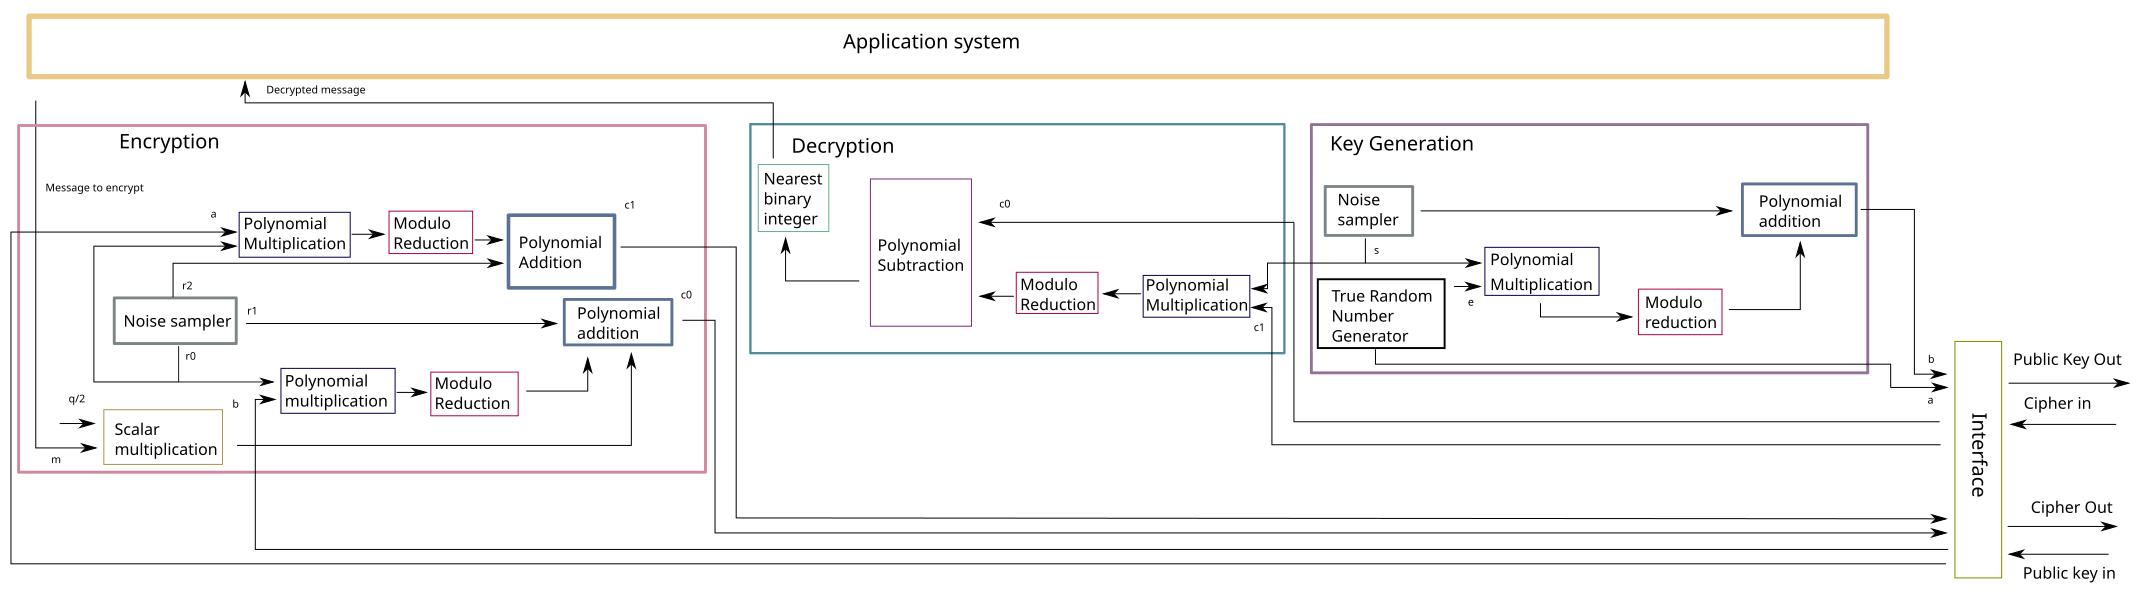
\includegraphics[scale=0.15]{high_level_impl.png}
    \caption{Hög nivå implementering av LMF \citep{FPGA_post_quantum}}
    \label{fig:high_level_impl}
\end{figure}

I Figur \ref{fig:high_level_impl} ser vi en hög nivå implementation av detta
kryptosystem. Men i denna essä kommer vi inte att gå in på hur \textit{True
Random Number Generator} fungerar samt inte heller hur \textit{Noise Samplern}
fungerar. Vi har försökt undvika dyra operationer som modulo då de tar väldigt
många uppslags tabeller.

\textit{Polynomisk addition/subtraktion} är implementerat med hjälp
av att göra operationen komponentvis och använt sig av villkorlig lagring
för att undvika modulära operationer. I Figur \ref{fig:pol_add} ser vi en
implementation av detta.

\begin{figure}[H]
    \centering
    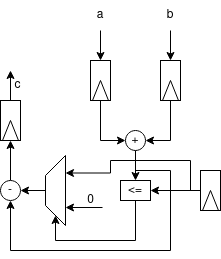
\includegraphics[scale=0.5]{images/polynomial_addition.png}
    \caption{Polynomisk addition}
    \label{fig:pol_add}
\end{figure}

I Figur \ref{fig:scal_mul} implementerar vi \textit{skalär multiplikation}. Då
vi räknar $t\cdot m$ väljer vi i princip $t$ eller $0$. Detta är möjligt för att
$m$ är en $n$-bit vektor. På grund av det kan vi igen använda oss av
villkorlig lagring för att undvika användning av modulo.

\begin{figure}[H]
    \centering
    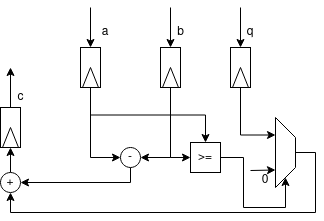
\includegraphics[scale=0.5]{images/scalar_multiplication.png}
    \caption{Skalär multiplikation}
    \label{fig:scal_mul}
\end{figure}

Låt $g = (c_0 - c_1 \cdot s)$, då vi räknar
\textit{skalär division till närmaste heltal} så kan vi använda oss av att
närmaste heltal kommer att vara $|g - t| < \frac{t}{2} \quad ? \quad 1 \quad :
\quad 0$. Detta är på grund av att $|g - t|$ beräknar distansen mellan $g$ och
$t$, om resultatet är större än halva $t$ så är de långt ifrån varandra och
kvoten kommer att vara 0. Å andra sidan om de är nära varandra så kommer
kvoten att vara 1.

\begin{figure}[H]
    \centering
    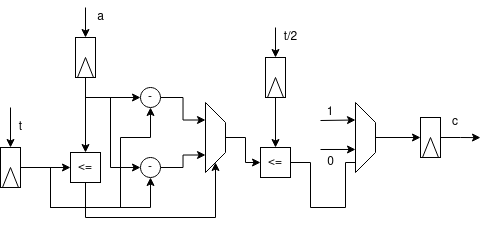
\includegraphics[scale=0.5]{images/scalar_division.png}
    \caption{Skalär multiplikation}
    \label{fig:scal_div}
\end{figure}

\textit{Polynomisk multiplikation} är den mest komplexa delen i vår design.
Vi använder oss av \textit{Talteoretiska Transformen} (TTT) för att göra
multiplikation snabbare. TTT är en generaliserad form av diskreta
fouriertransformen över ringen $R_q = \bZ_q[X] / \langle X^n + 1 \rangle$. TTT
definieras på följande sätt: låt $\omega$ vara $n$te enhetsroten för polynomet

\[ X_i = \sum_{k=0}^{n-1}x_k \cdot \omega^{ik}. \]

\begin{figure}[H]
    \centering
    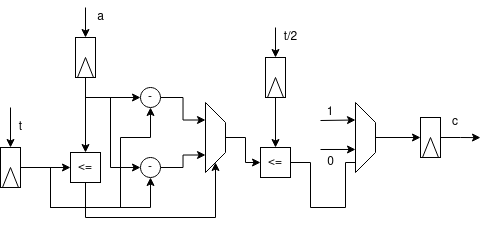
\includegraphics[scale=0.5]{images/scalar_division.png}
    \caption{Skalär multiplikation}
    \label{fig:pol_mul}
\end{figure}
I normala fall då man multiplicerar komponenterna har multiplikation en
komplexitet av $\mathcal{O}(n^2)$ men med TTT är komplexiteten
$\mathcal{O}(n\log n)$. För mera detaljer om hur TTT är implementerat, se
\citep{FPGA_post_quantum}.

Hårdvarokostnaderna ser vi i Tabell \ref{tab:hardwarecost}. Dessa
implementationer är även circa 22\% till 78\% snabbare än tidigare
implementationer \citep{FPGA_post_quantum}.

\begin{table}[H]
    \centering
    \begin{tabular}{l|ll}
        \textit{n} & UTn   & Register \\ \hline
        128        & 66251  & 16805     \\
        256        & 11490  & 33138     \\
        512        & 227458 & 65643     \\
        1024       & 426402 & 130540
    \end{tabular}
    \caption{Hardware cost using only LUTs where $q = 12289$
    \citep{FPGA_post_quantum}}
    \label{tab:hardwarecost}
\end{table}

\printbibliography

\end{document}
